\subsubsection{Comparison of featuresets  \label{compoffeatureset}}

The best configurations of the experiments using the Bertsekas
featureset never appears to score much higher than 200,000 lines
on average. Due to this, the question of whether the specific featureset
causes rapid convergence remains.\\
To address this, both CMA-ES and Cross
Entropy experiments were run 30 times with respectively the Bertsekas and 
Dellacherie featureset. To prevent long runtimes, the games were simulated
using a harder version of Tetris referred to as 'Hard Tetris'. With regular 
Tetris, all pieces occur with equal likelihood.\\
%(see figure \ref{fig:TetrisPieces})
To increase the difficulty of the game,
in our hard Tetris, the s-block and z-block appear twice as often 
as the other pieces.

\begin{figure}[H]
\begin{center}
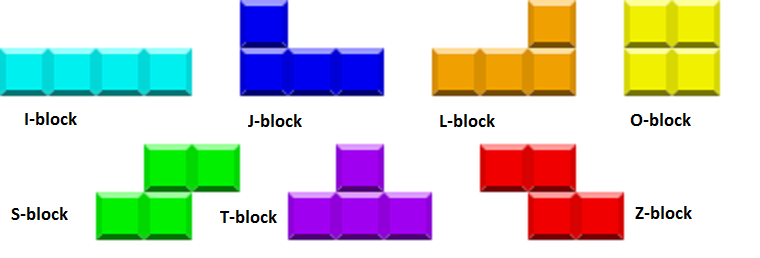
\includegraphics[scale=0.6]{img/Pieces}
\end{center}
\caption{Regular Tetris pieces \label{fig:TetrisPieces}}
\end{figure}

\textbf{Results}

In the following figures the mean results of 30 runs of both CMA and Cross 
Entropy is presented. The settings for Cross Entropy remains at constant noise
with a noise term of $z_t = 4$ and an initial sigma of $\sigma_0 = 100.$, 
and the CMA with $\sigma_0 = 1$.\\
\\
Figure \ref{fig:featuresetCompareBertsekas} shows the experiment with the 
Bertsekas featureset. This shows that when running the algorithms with a
harder game, the algorithms behave mostly the same as with regular 
Tetris. Namely that CMA converges faster than Cross Entropy, 
but is eventually outperformed.

\begin{figure}[H]
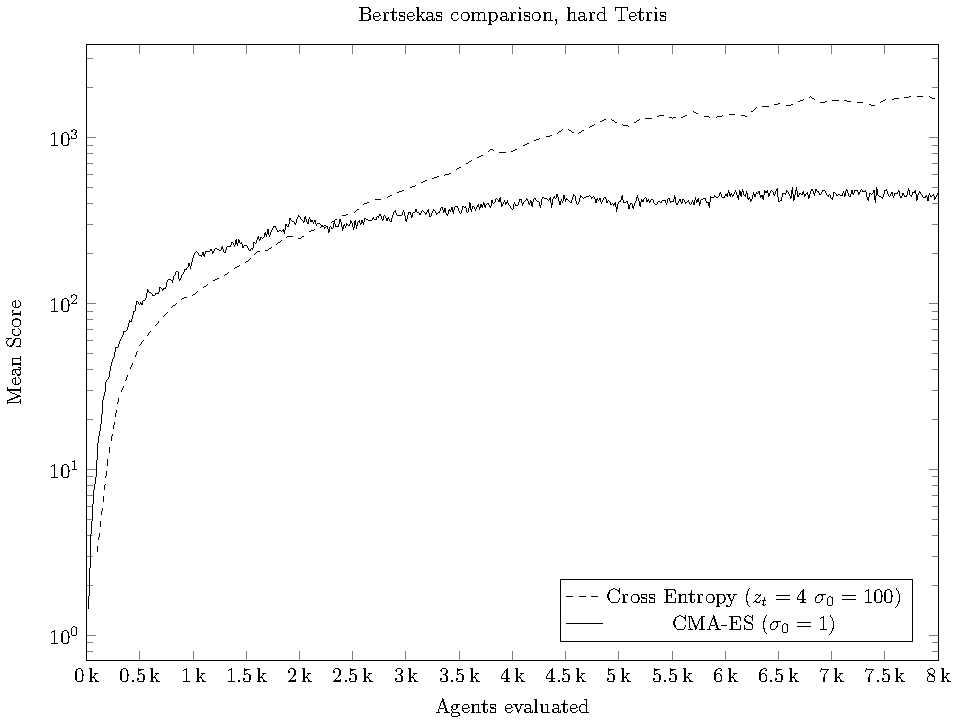
\includegraphics[scale=1]{plots/plotBertsekasCmaVsCEHardTetris}
\caption{Comparison between CMA-ES and Cross Entropy 
using hard Tetris and the Bertsekas featureset 
\label{fig:featuresetCompareBertsekas}}
\end{figure}

When using the Dellacherie featureset a similar behaviour is observed.
However, the convergence seems to occur earlier and with a higher score
(figure \ref{fig:featuresetCompareDellacherie}).

\begin{figure}[H]
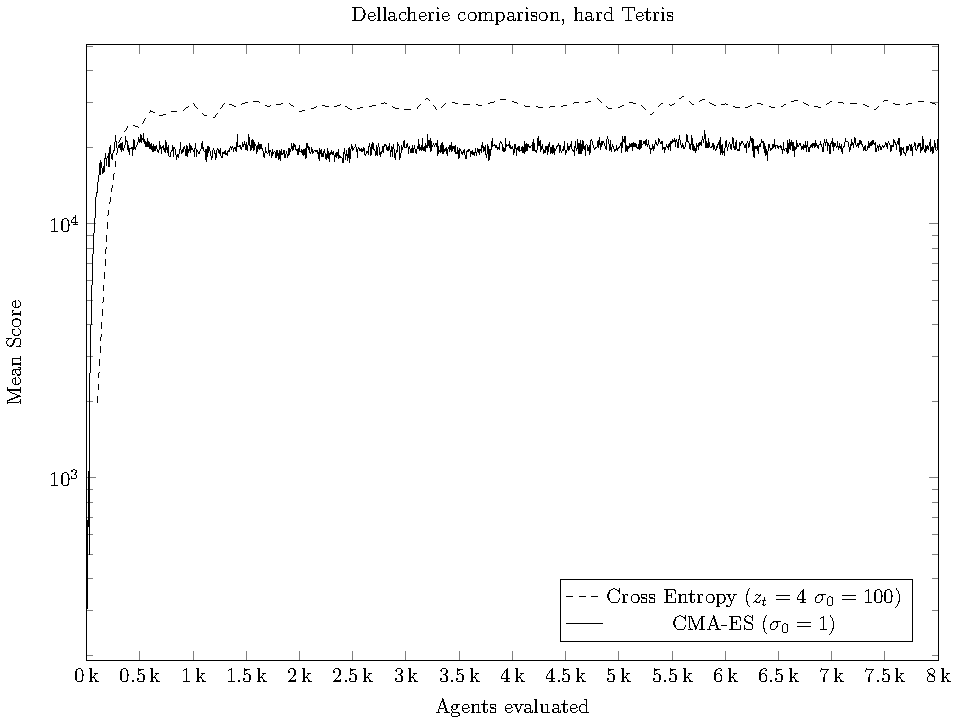
\includegraphics[scale=1]{plots/plotDellCmaVsCEHardTetris}
\caption{Comparison between CMA-ES and Cross Entropy 
using hard Tetris and the Dellacherie featureset
\label{fig:featuresetCompareDellacherie}}
\end{figure}

\comment
{
Add full data graphs as appendix.
}



\textbf{Analysis and discussion}

The experiment with different featuresets indicates that the behaviour 
is not heavily dependant on the featureset, as the development of the 
graphs closely resemble the initial comparison experiment.
Furthermore, it appears that increasing the difficulty of the game
simple shifts the score, but does not affect the development of the graphs.
Therefore, we conclude that changing the featureset does not invalidate
the comparison of the two optimization algorithms. In further experiments,
in our configuration of CMA, the harder version of Tetris is applied
in experiments used to optimize the CMA configurations.\\
\comment{This conclusion doesn't make kronologisk sense}